\documentclass[14pt, a4paper]{article}
\usepackage{float}
\usepackage{graphicx}
\usepackage[utf8]{inputenc}
\usepackage[margin=1in]{geometry}

\DeclareGraphicsExtensions{.png}

\begin{document}

%\title and intnro
\begin{titlepage}
	\begin{center}
		
		\begin{figure}[t]
			\centerline{
			
\includegraphics[width=450px]{./Graphics/KPTH_Logo.png}}
		\end{figure}		
		
		\textbf{\LARGE Gynaecological Patient Information
		management System:}
		
		\vspace{1 cm}
	    \textbf{\LARGE \\User Manual}
		
		\vspace{1 cm}
		\LARGE{\textbf{Team Pentec: }}
		

		\begin{flushright} \large
			
			Ruth Ojo 12042804\newline
			Liz Joseph 10075268\newline
			Trevor Austin 11310856\newline
			Maria Qumayo 29461775\newline
			Lindelo Mapumulo 12002862\newline
		\end{flushright}
		
				\vspace{1 cm}
				\centering
				
\includegraphics[width=150px]{./Graphics/Pentec_Logo.png}

		
		{\LARGE Version 1.4} 
		\\
		{\large \today}		
		
		
	\end{center}
\end{titlepage}


\begin{abstract}
\Large
This document is the Software User Manual (SUM) for the Patient Information Management System project and was made according to the software engineering standard described in the tender proposal provided by Professor Snyman. The Software User Manual (SUM) instructs how to install and use the
Patient Information Management System software. This project is part of the Software Engineering Project course (COS301) at the University of Pretoria.\\
\end{abstract}

\newpage

%\table of content
\tableofcontents
\newpage

\section{Introduction}


\subsection{Change Log}
Document Title: Software User Manual\\
Version: 0.1.0\\
Document Status: conditionally approved\\
Version Date Author(s) Summary\\
0.0.1 29-05-2015 LN. Joseph Document creation\\


\subsection{Intended readership}
This document covers the use for the following users of the PIMS system:\\
\begin{description}
\item the system administrator
\item the project administrators
\item the medical staff
\item the usability test subjects
\end{description}

\subsection{Applicability}
This Software User Manual (SUM) applies to the PIMS software, version 0.1.\\


\subsection{Purpose}
The purpose of the SUM is to assist the user in installing and using the PIMS software.\\

	
\subsection{How to use this document}
\begin{description}
\item How it is to be used:
\item[$\bullet$] Title page - System name and the names and/or affiliation of all stakeholders.
\item[$\bullet$] Introduction - Introduction to the System
\item[$\bullet$] Overview - Purpose of the system
\item[$\bullet$] Configuration - Configuration used by the system
\item[$\bullet$] Installation - Detailed description of where to find the software and how to install it.
\item[$\bullet$] Getting Starting - Walk through of the system
\item[$\bullet$] Using the System - Description of the systems functions
\item[$\bullet$] Troubleshooting - Procedures to take in case of errors
\end{description}

	
\subsubsection{Problem Reporting}
Since the Pentec team will be dissolved after completion of the PIMS project, the
issue of problem reporting is left to the Administrator, Professor Snyman.\\
	
	
\newpage

\section{Overview}
The purpose of this software is to be used by doctors and medical staff. It allows the administrative users to electronically fill in medical forms and be able to query for statistics for those forms and eventually receive a prediction that could assist in the functionality of the Kalafong Hospital. Regular users are allowed to fill in medical forms.
\\

\newpage

\section{Configuration}
\subsection{System Configuration}
\subsubsection{Basic System Structure}
The current system that is in place makes use of a Node.js server that interacts with any web client. The server is hosted through a PaaS named Heroku. The system delivers compiled jade files to the users that are stylized using CSS. The jade files are controlled and animated by Javascript and jQuery. The node.js server accesses MongoDB database hosted on the DaaS, mongolab. This is illustrated below:
\begin{figure}[h!]
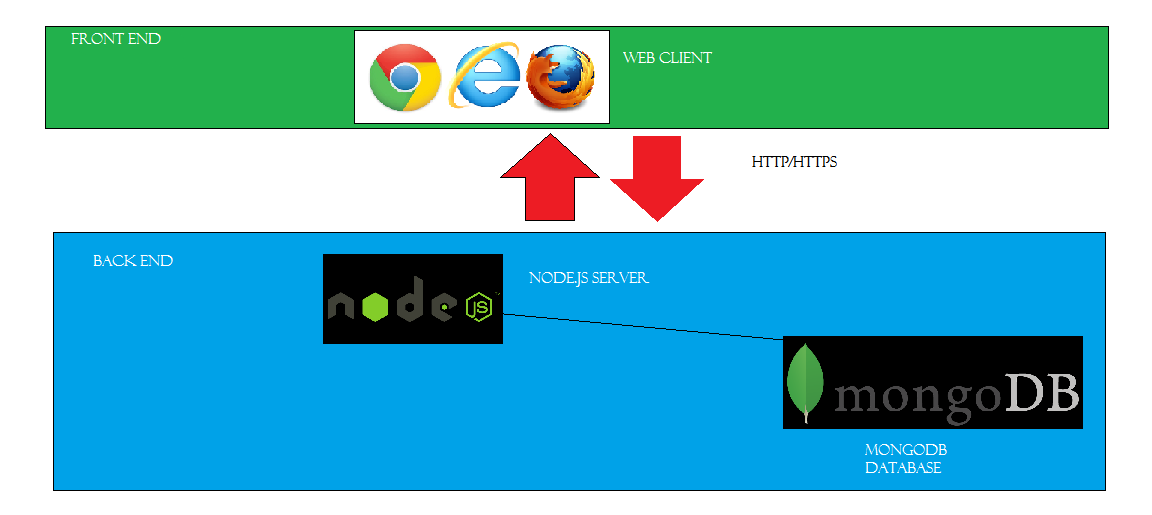
\includegraphics[width=1.0\textwidth]{Graphics/Screenshots/infrastructure}
\end{figure}
\newpage
\subsubsection{Node.js Architecture}
Node.js is an asynchronous langauge and its basic client-server communication is illlustrated below:
\begin{figure}[h!]
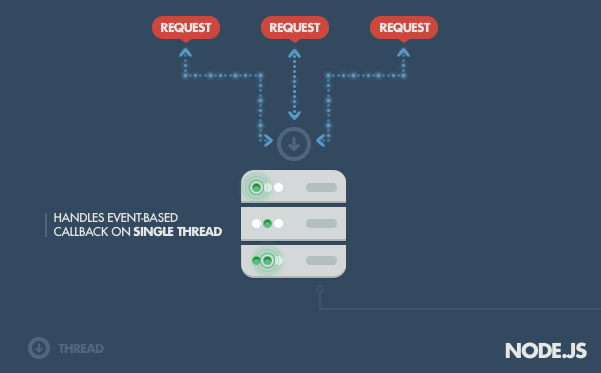
\includegraphics[width=1.0\textwidth]{Graphics/Screenshots/nodejsinfrastructure}
\end{figure}
\subsubsection{Communication Protocols Used}
This is the current list of all communication protocols used by PIMS:
\begin{itemize}
	\item HTTP/HTTPS
	\item SMTP
\end{itemize}
\newpage

\newpage


\section{Installation}
\subsection{Running the Software}
\begin{enumerate}
  \item Website page
  \begin{enumerate}
  \item Establish an internet connection
    \item Search for website in web browser
    \item Log into PIMS system with given authentication codes
  \end{enumerate}
  \item Mobile Application
   \begin{enumerate}
   \item Establish an internet connection
    \item Search for website in web browser
    \item Log into PIMS system with given authentication codes
  \end{enumerate}
  \item Tablet or other
   \begin{enumerate}
\item Establish an internet connection  
    \item Search for website in web browser
    \item Log into PIMS system with given authentication codes
  \end{enumerate} \ldots
\end{enumerate}

\subsection{Shutting down the website}
Contact your service provider(hosting site) to pull down the software
\newpage


\section{Getting Started}
\subsection{Systems Procedure Order}
This section describes a brief overview of how a user can access the system, it shows perspectives from an adminstrative user as well as normal users. The sections that are discussed can be found in more detail in the next section.
\subsection{Splash Page}
	\begin{figure}[H]
		\fbox{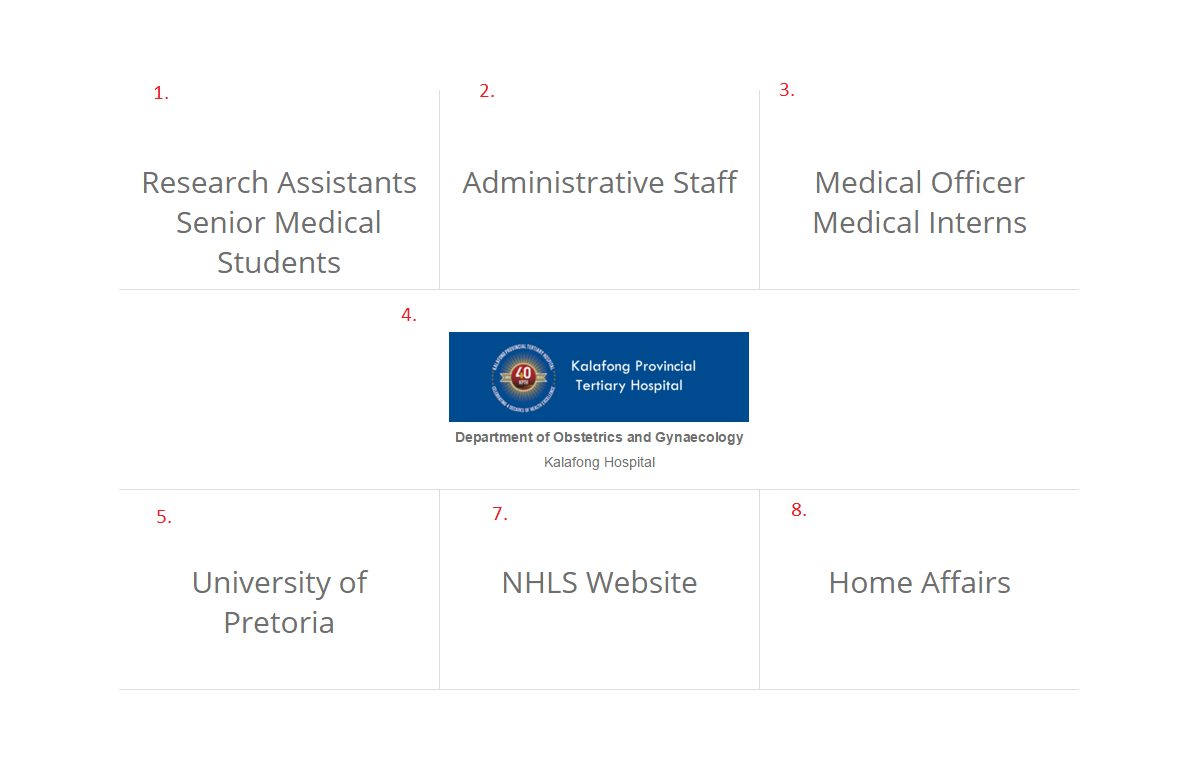
\includegraphics[width=1.0\textwidth]{Graphics/Screenshots/splash}}
		\caption{The splash page.}
  		\label{fig:splash1}
	\end{figure}
	\subsubsection{Description}
		This section links users to different pages that they can access. A more detailed description of each component can be found below.
	\subsubsection{Detailed Component Description}
		\begin{enumerate}
			\item \textbf{Research Assistants \& Senior Medical Students Link:} This is a link that will direct the user to a customized login page for research assistants and senior medical students.
			\item \textbf{Administrative Staff Link:} This is a link that will direct the user to a customized login page for administrative staff.
			\item \textbf{Medical Officer \& Medical Interns Link:} This is a link that will direct the user to a customized login page for medical officers and medical interns.
			\item \textbf{Kalafong Hospital Link:} This link directly links users to the official University of Pretoria Kalafong hospital page.
			\item \textbf{University of Pretoria Link: } This link directly links users to the official university of pretoria page.
			\item \textbf{National Health Laboratory Service Link:} This is a link that will direct users to NHLS website.
			\item \textbf{Home Affairs Link:} This is a link that will direct users to the home affairs website in order to allow users to check their life status.
		\end{enumerate}
	\subsubsection{Accessing user login}
		\begin{enumerate}
			\item Select the link that is relative to user's login. Eg. Research Assistants should click the Researh Assistants \& Senior Medical Students link.
			\item More information on the login page in the login tutorial section\ldots
		\end{enumerate}
\subsection{Login}
	\begin{figure}[H]
		\fbox{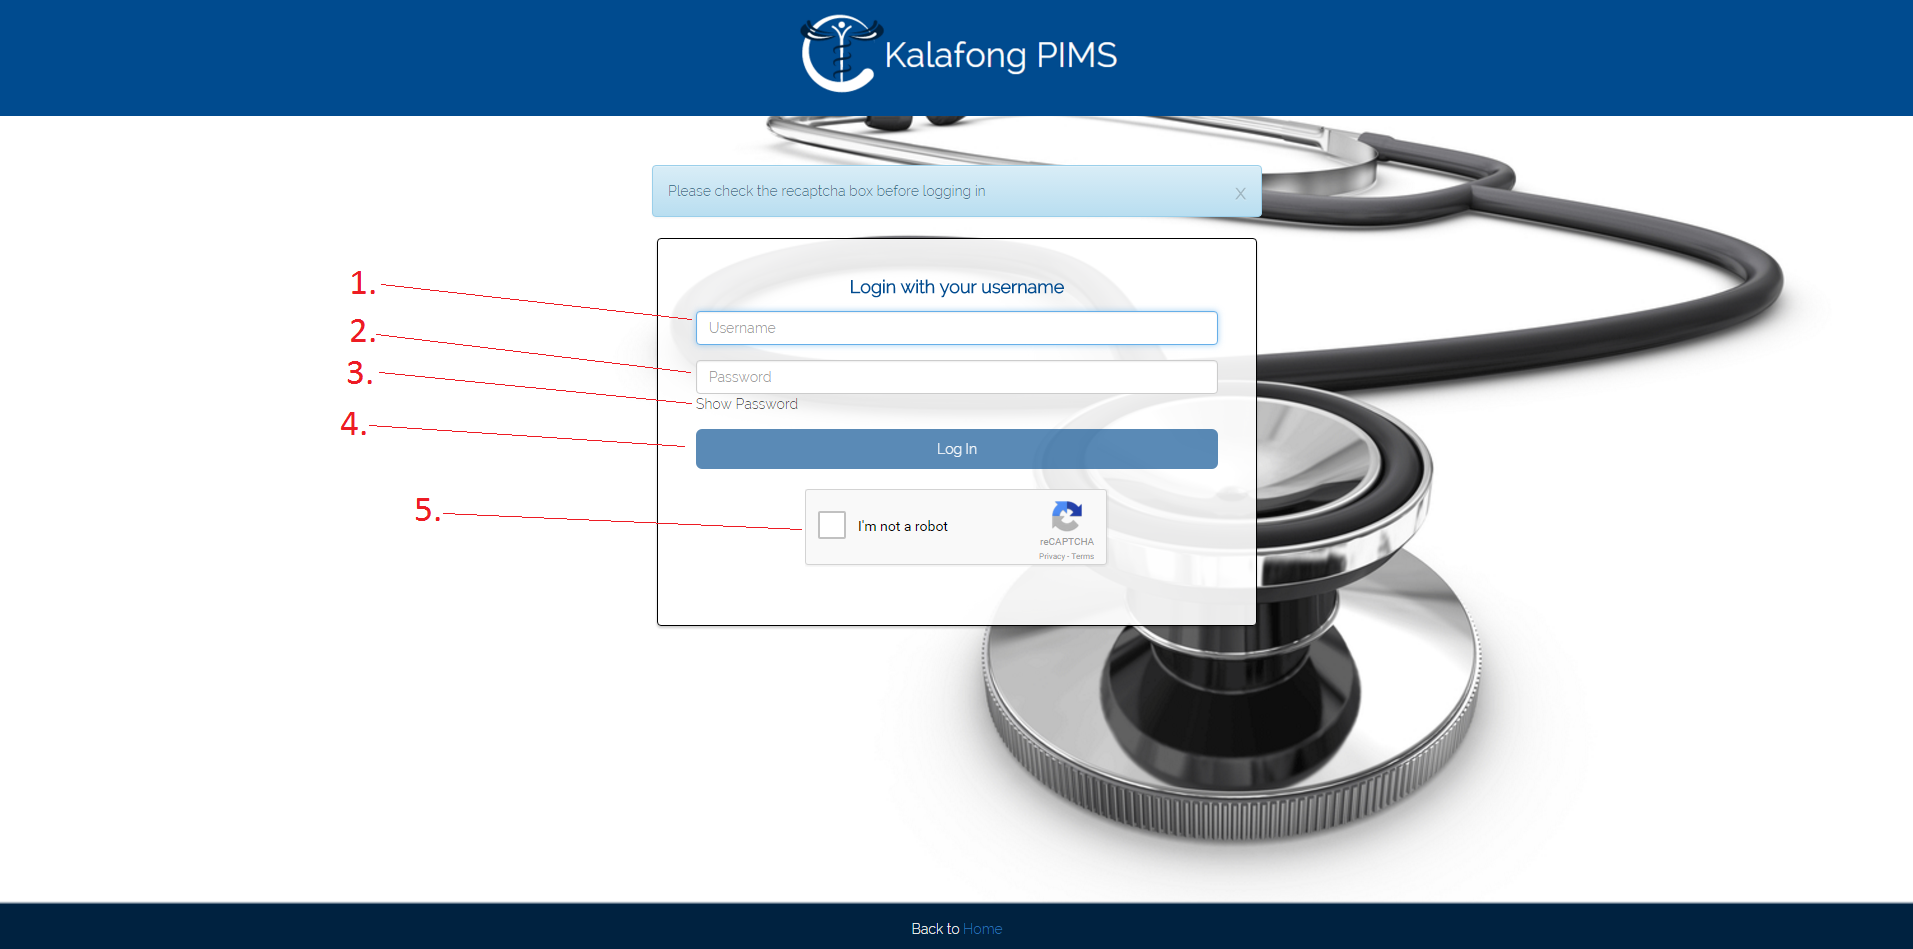
\includegraphics[width=1.0\textwidth]{Graphics/Screenshots/loginMain}}
		\caption{The login page.}
  		\label{fig:login1}
	\end{figure}
	\subsubsection{Description}
		This is the login page that all users must access before being able to access the main web page. Users must fill in their credentials and pass a security check to be able to access this page. More detailed information can be found below.
	\subsubsection{Detailed Component Description}
		\begin{enumerate}
			\item \textbf{Username Input Box:} This is the input box in which users will enter in their username.
			\item \textbf{Password Input Box:} This is the input box in which users will enter in their password.
			\item \textbf{Show Password Button:} This button allows users to check their password text. Clicking this button will toggle between whether the password is shown or not.
			\item \textbf{Login Button:} This is the button the users will click once they have filled in their information and passed the security check. This will link them to their relative my space page.
			\item \textbf{Recaptcha: } This is the security check that is put in place. More information on how to use it is placed within the \textit{"How to Login"} section.
		\end{enumerate}
		\subsubsection{How to login}
		\begin{enumerate}
			\item Fill in username input box and confirm it is correct. NOTE: If the user login page does not look like the above do not panic. There are different themes for each user type. The other themes can be found at the bottom of the login section in figure \ref{fig:login2}.
			\item Fill in password input box and confirm it is correct. The user can confirm the password is correct using the show password button.
			\item Complete the security check for the recaptcha by clicking on the recaptcha checkbox.
			\item If multiple logins have been made in succession, a user may be prompted to select certain images related to a theme. For example, below (Figure \ref{fig:recaptcha1}) the recaptcha is asking the user to select all images with street signs.
			\begin{figure}[H]
				\centerline{\fbox{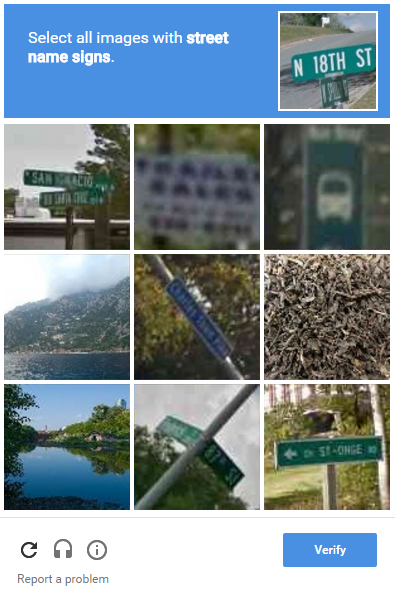
\includegraphics[width=0.3\textwidth]{Graphics/Screenshots/recaptchaFill}}}
				\caption{Recaptcha prompt.}
  				\label{fig:recaptcha1}
			\end{figure}
			\item If the recaptcha security check is successful the checkbox will look like figure \ref{fig:recaptcha2}.
			\begin{figure}[H]
				\centerline{\fbox{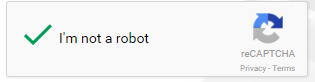
\includegraphics[width=0.3\textwidth]{Graphics/Screenshots/recaptchaCorrect}}}
				\caption{Passed recaptcha security check.}
  				\label{fig:recaptcha2}
			\end{figure}
			\item The user will now be able to click the login button to redirect them to their MyPimsSpace page.
		\end{enumerate}
	\begin{figure}[H]
		\fbox{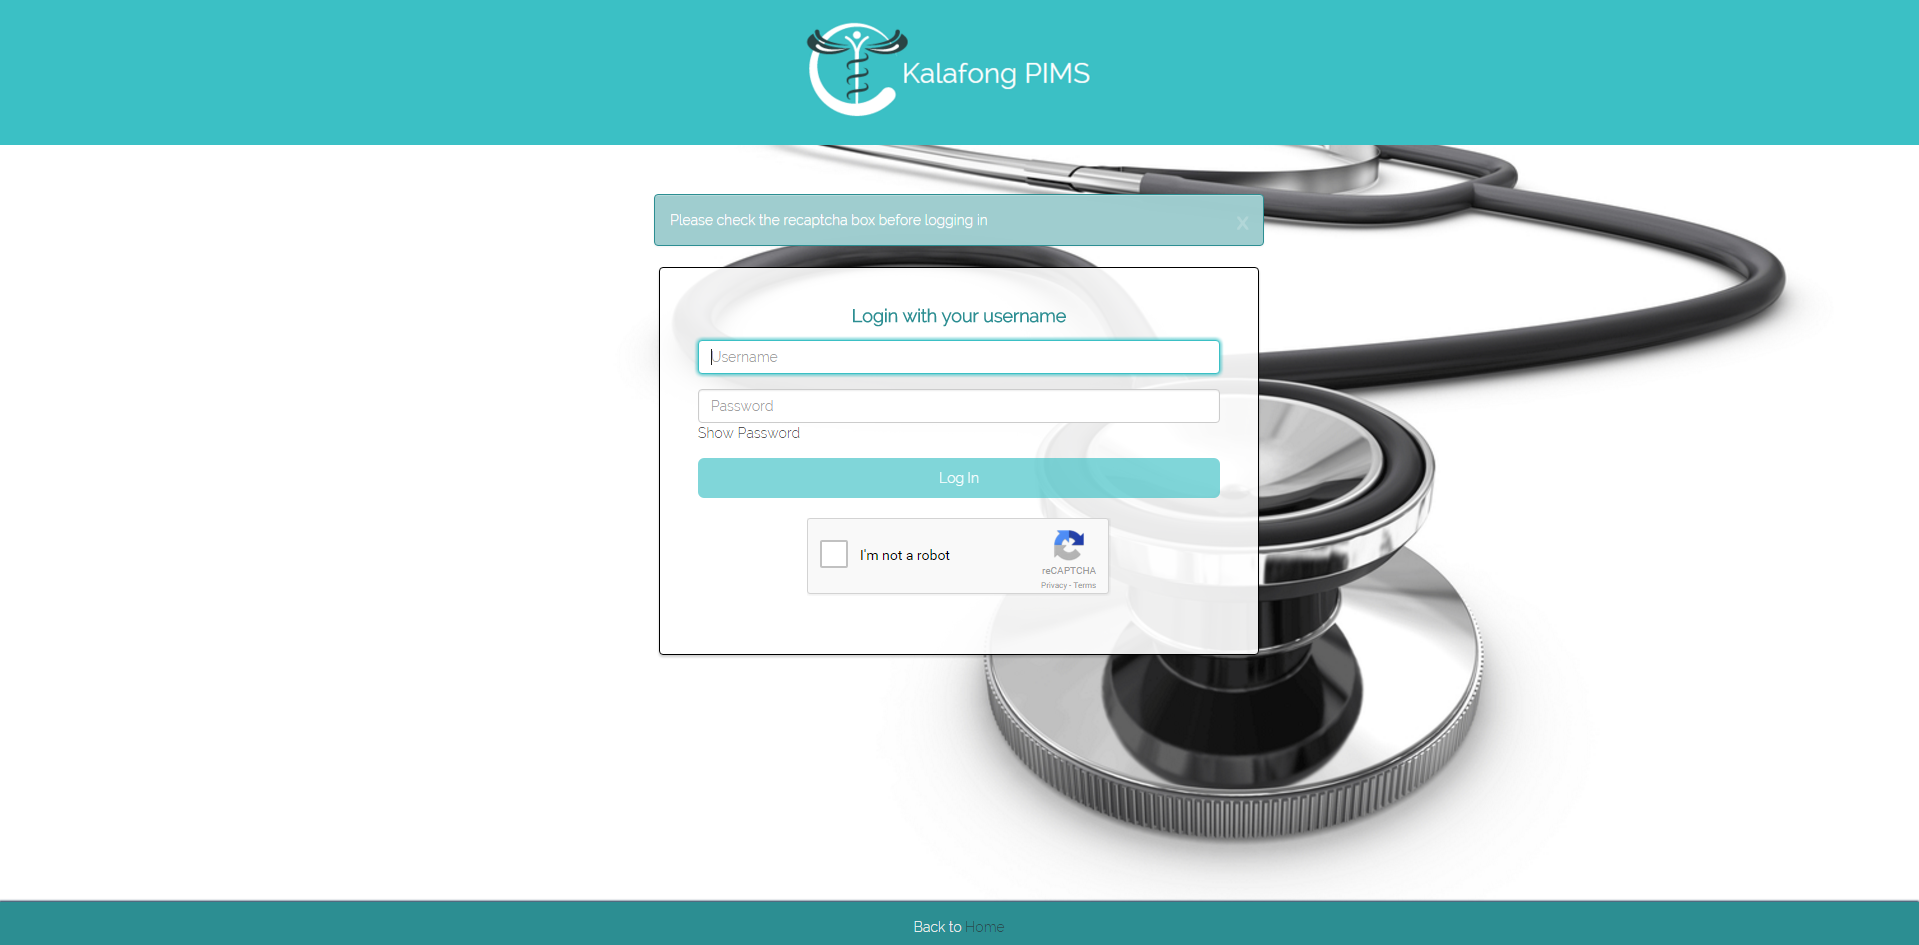
\includegraphics[width=0.5\textwidth]{Graphics/Screenshots/loginI}}
		\fbox{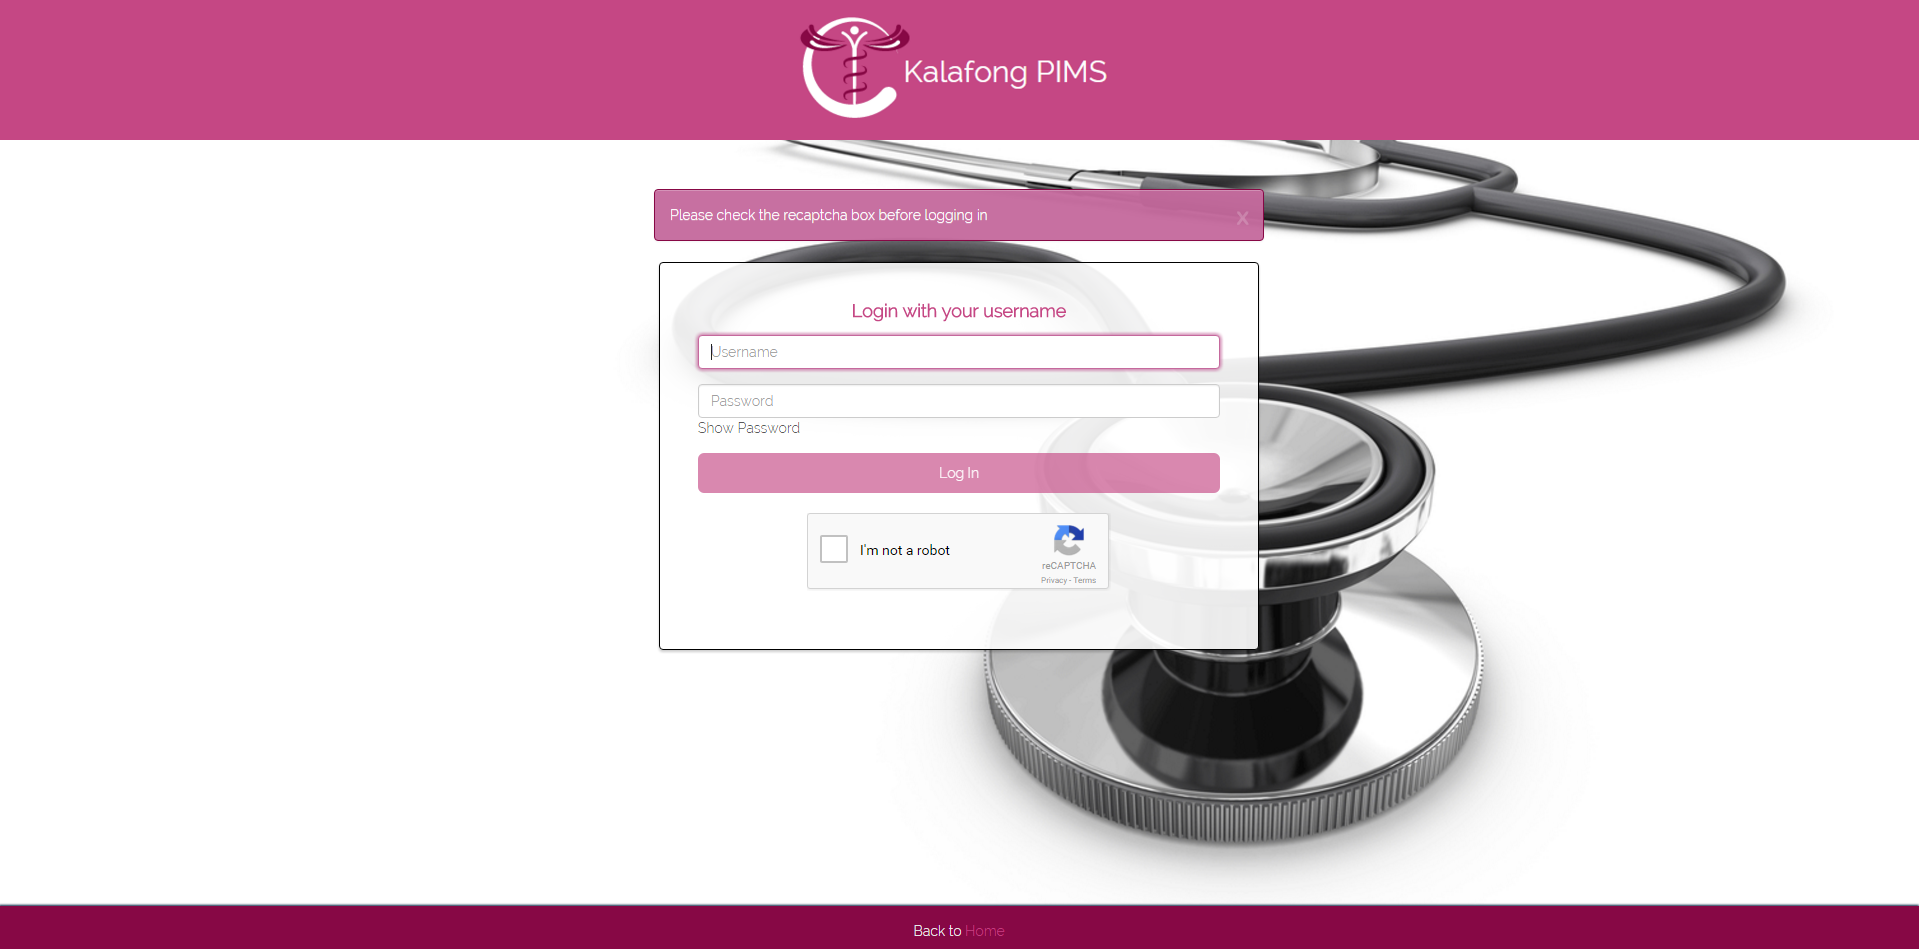
\includegraphics[width=0.5\textwidth]{Graphics/Screenshots/loginR}}
		\caption{Other themed login pages.}
  		\label{fig:login2}
	\end{figure}
\newpage
\subsection{Admin Navbar}
	\begin{figure}[H]
		\fbox{
\includegraphics[width=1.0\textwidth]{Graphics/Screenshots/navbar}}
		\caption{The Admin Navbar.}
  		\label{fig:navbar1}
	\end{figure}
	\subsubsection{Description} This is the navbar that administrative users will use to help them navigate through pages with ease. A more detailed description can be found below.
	\subsubsection{Detailed Component Description}
		\begin{enumerate}
			\item \textbf{Logo:} This is the logo for the kalafong PIMS and if clicked willl link the user back to their MyPimsSpace page.
			\item \textbf{Active tab:} This is the active tab and will identify to user the current page that are on using a dark blue line at the bottom of its tab. If clicked it will reload the current page. (NOTE: If tab has sub-tabs it willl behave as a Submenu tab).
			\item \textbf{Submenu tab:} This is a submenu tab and when clicked willl reveal sub tabs that relate to the sub menu tab.
			\item \textbf{Subtab:} Behave like regular tabs but do not underline when active, instead the Submenutab will be underlined.
			\item \textbf{Dropdown tab: } This is a dropdown tab and when click willl display a dropdown menu much the like the one in figure \ref{fig:navbar1}.
			\item \textbf{Regular tab: }  These tabs will link a user to the specified section. Eg. Predict will link the user to the prediction page.
			\item \textbf{Settings tab:} This tab works similar to a submenu tab and can show all the optional settings for the specific user.
			\item \textbf{Logout tab:} This tab is a regular tab but when clicked the user will be logged out and redirected to the splash page.
		\end{enumerate}
	\subsubsection{How to navigate a Subtab}
		\begin{enumerate}
			\item Click on the Submenu tab which willl reveal the Subtabs with an animation
			\item Click on the subtab which is relevant to the page the user would like to access. Then the user will then be redirected to that page.
			\begin{figure}[H]
				\centerline{\fbox{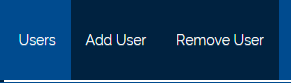
\includegraphics[width=0.4\textwidth]{Graphics/Screenshots/activeNavbar}}}
				\caption{Submenu tab with subtabs visible}
  				\label{fig:navbar2}
			\end{figure}
		\end{enumerate}
	\subsubsection{How to navigate a dropdown menu}
		\begin{enumerate}
			\item Click on the Submenu tab which willl reveal the dropdown menu.
			\item Click on the dropdown tab which is relevant to the page the user would like to access. Then the user will then be redirected to that page.
			\begin{figure}[H]
				\centerline{\fbox{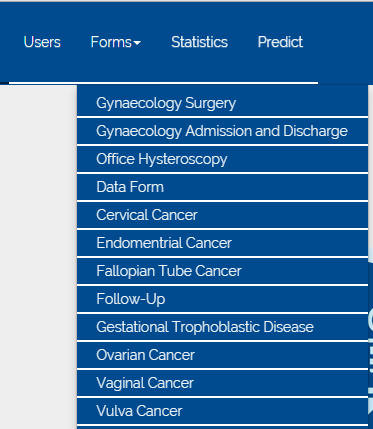
\includegraphics[width=0.4\textwidth]{Graphics/Screenshots/navbarDropdown}}}
				\caption{Dropdown menu}
  				\label{fig:navbar3}
			\end{figure}
		\end{enumerate}
	\subsubsection{How to navigate a regular tab}
		\begin{enumerate}
			\item Click on the regular tab which is relevant to the page the user would like to access. Then the user will then be redirected to that page.
		\end{enumerate}
	\subsubsection{How to navigate the settings tab}
		\begin{enumerate}
			\item Click on the Settings tab which willl reveal the Subtabs with an animation
			\item Click on the subtab which is relevant to the page the user would like to access. Then the user will then be redirected to that page.
			\begin{figure}[H]
				\centerline{\fbox{
\includegraphics[width=0.4\textwidth]{Graphics/Screenshots/activeSettings}}}
				\caption{Active settings menu}
  				\label{fig:navbar3}
			\end{figure}
		\end{enumerate}
	\subsubsection{How to Logout}
		\begin{enumerate}
			\item Click the logout tab and the user will be logged out.
		\end{enumerate}
\subsection {Regular User Navbar}
	\begin{figure}[H]
		\fbox{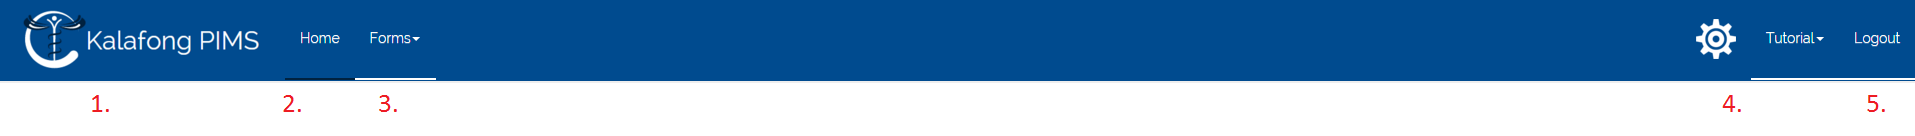
\includegraphics[width=1.0\textwidth]{Graphics/Screenshots/navbarUser}}
		\caption{The User Navbar.}
  		\label{fig:navbar4}
	\end{figure}
	\subsubsection{Description} This is the navbar that users will use to help them navigate through pages with ease. A more detailed description can be found below.
	\subsubsection{Detailed Component Description}
		\begin{enumerate}
			\item \textbf{Logo:} This is the logo for the kalafong PIMS and if clicked willl link the user back to their MyPimsSpace page.
			\item \textbf{Active tab:} This is the active tab and will identify to user the current page that are on using a dark blue line at the bottom of its tab. If clicked it will reload the current page. (NOTE: If tab has sub-tabs it willl behave as a Submenu tab).
			\item \textbf{Dropdown tab: } This is a dropdown tab and when click willl display a dropdown menu much the like the one in figure \ref{fig:navbar1}.
			\item \textbf{Settings tab:} This is a settings tab and when clicked willl reveal sub tabs that relate to the sub menu tab.
			\item \textbf{Logout tab:} This tab is a regular tab but when clicked the user will be logged out and redirected to the splash page.
		\end{enumerate}
	\subsubsection{How to navigate a dropdown menu}
		\begin{enumerate}
			\item Click on the Submenu tab which willl reveal the dropdown menu.
			\item Click on the dropdown tab which is relevant to the page the user would like to access. Then the user will then be redirected to that page.
			\begin{figure}[H]
				\centerline{\fbox{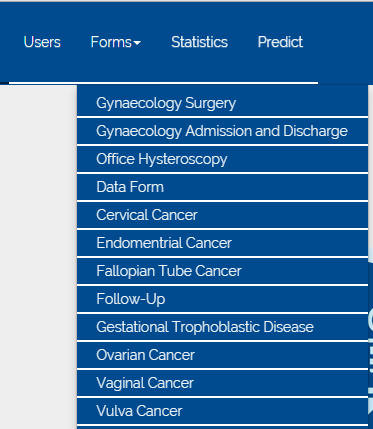
\includegraphics[width=0.4\textwidth]{Graphics/Screenshots/navbarDropdown}}}
				\caption{Dropdown menu}
  				\label{fig:navbar5}
			\end{figure}
		\end{enumerate}
	\subsubsection{How to navigate a regular tab}
		\begin{enumerate}
			\item Click on the regular tab which is relevant to the page the user would like to access. Then the user will then be redirected to that page.
		\end{enumerate}
	\subsubsection{How to navigate the settings tab}
		\begin{enumerate}
			\item Click on the Settings tab which willl reveal the Subtabs with an animation
			\item Click on the subtab which is relevant to the page the user would like to access. Then the user will then be redirected to that page.
			\begin{figure}[H]
				\centerline{\fbox{
\includegraphics[width=0.4\textwidth]{Graphics/Screenshots/activeSettings}}}
				\caption{Settings menu. NOTE: This is the admin's settings menu and edit profile is not included in the regular users setting's subtabs.}
  				\label{fig:navbar6}
			\end{figure}
		\end{enumerate}
	\subsubsection{How to Logout}
		\begin{enumerate}
			\item Click the logout tab and the user will be logged out.
		\end{enumerate}
\subsection{Home Icons}
	\begin{figure}[H]
		\fbox{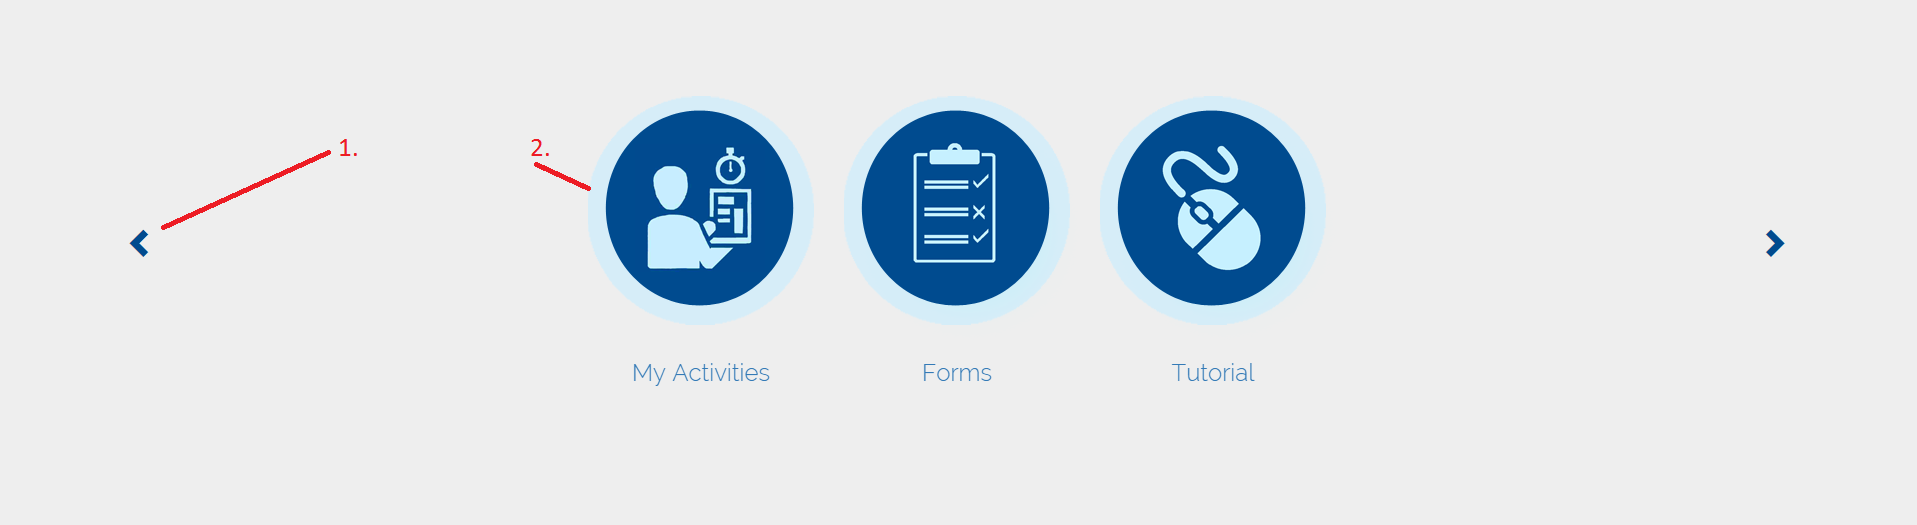
\includegraphics[width=1.0\textwidth]{Graphics/Screenshots/icons}}
		\caption{Admin \& User Home Icons}
  		\label{fig:icons1}
	\end{figure}
	\begin{figure}[H]
		\fbox{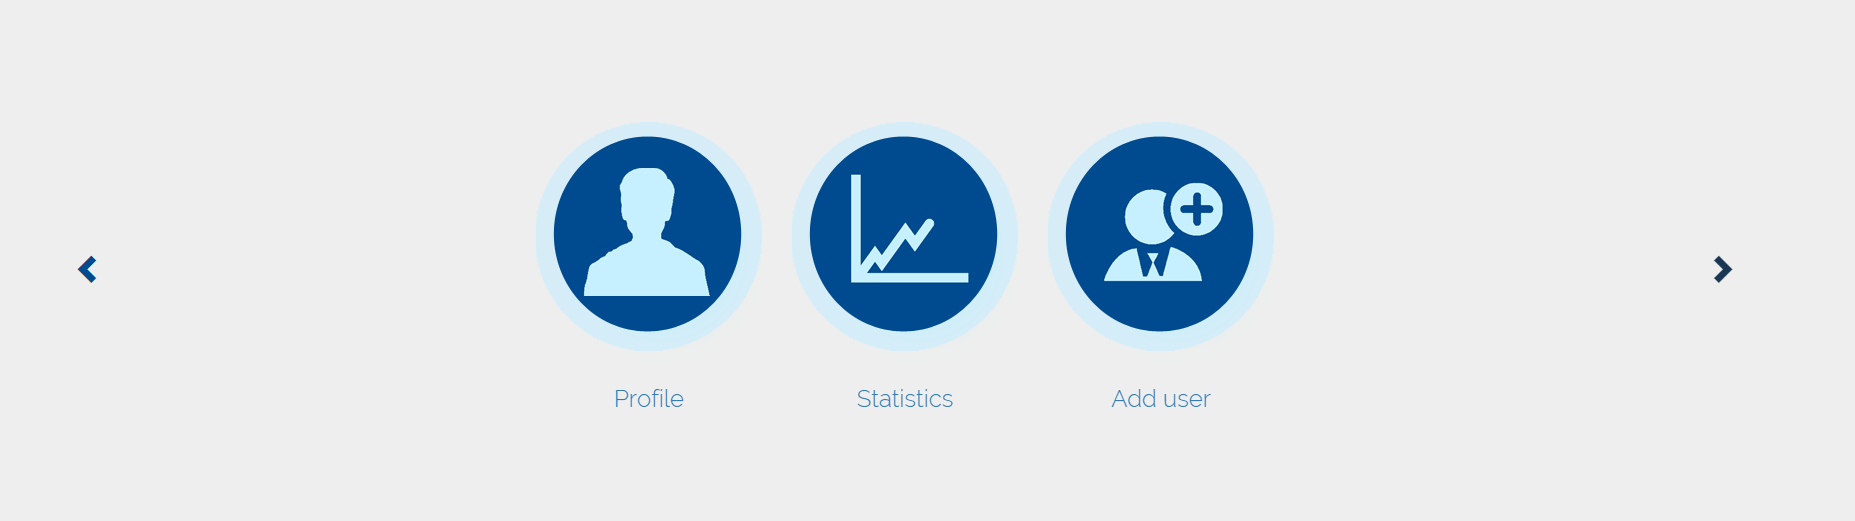
\includegraphics[width=1.0\textwidth]{Graphics/Screenshots/icons2}}
		\caption{More Admin Home Icons}
  		\label{fig:icons2}
	\end{figure}
	\subsubsection{Description} The home icons are put in place to ease up usability for users as well as provide an aesthetically pleasing way of navigating the web application. The animation in place is more aesthetic for a regular user as they have limited icons and thus can only navigate through the same set of icons.
	\subsubsection{Detailed Component Description}
		\begin{enumerate}
			\item \textbf{Navigation Arrow:} This arrow is used to navigate through the home icons.
			\item \textbf{Home icon:} This is used as a point of navigation, home icons can either be links or have have a submenu links.
		\end{enumerate}
	\subsubsection{How to navigate home icons}
		\begin{enumerate}
			\item By clicking the on the navigations arrows
		\end{enumerate}
		\begin{center} OR \end{center}
		\begin{enumerate}
			\item By clicking the left and right keyboard arrows
		\end{enumerate}
\subsection{Fill Forms}
	\begin{figure}[H]
		\centerline{\fbox{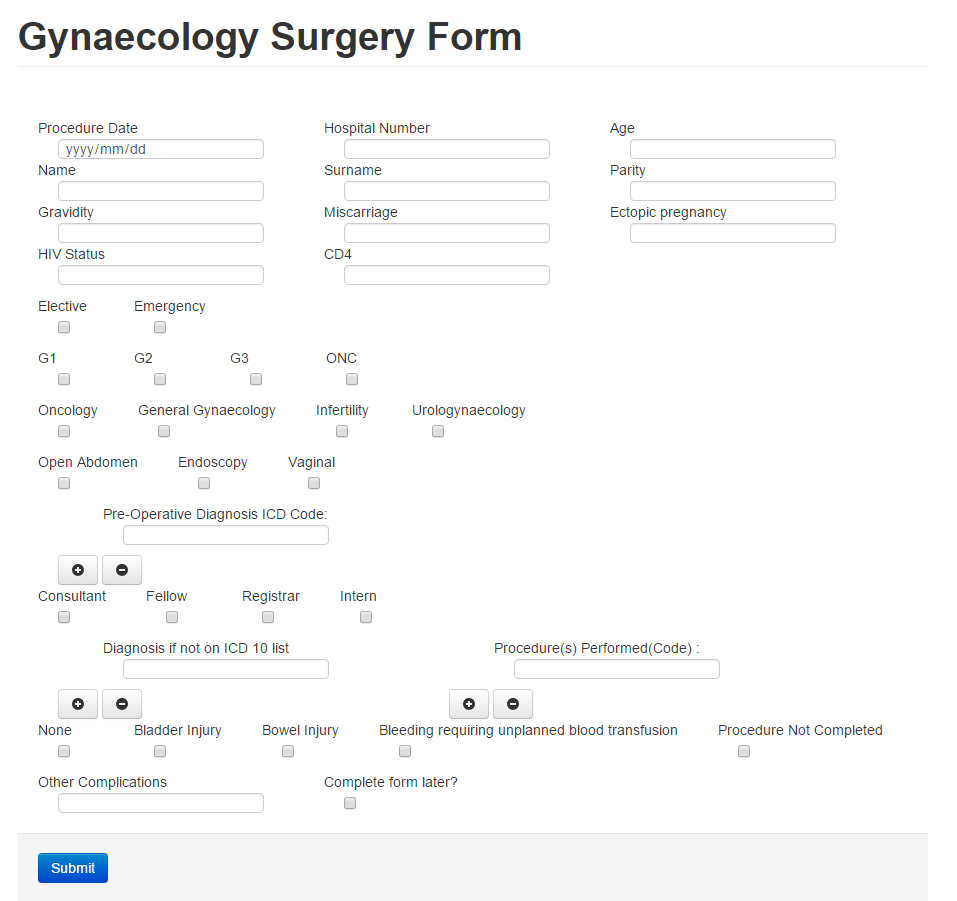
\includegraphics[width=0.8\textwidth]{Graphics/Screenshots/fillForms}}}
		\caption{An example of a form}
  		\label{fig:forms1}
	\end{figure}
	\subsubsection{Description} This section is where users can input data into the hospital forms for the system. 
	\subsubsection{Detailed Component Description}
		\begin{enumerate}
			\item \textbf{Input box:} This is an input field where users will place the required information needed for that field.
			\item \textbf{Check box:} This is check box in which users can check if the data collected meets the required checkbox.
			\item \textbf{ICD 10 input box:} This is an input box where users will place the required information needed for that field. Unlike regular input boxes these input boxes allow users to add and remove boxes using the + and - icons.
			\item \textbf{Submit button:} Users can click this button to submit the button once all information has been completed.
		\end{enumerate}
	\subsubsection{How to fill forms}
		\begin{enumerate}
			\item Fill in all required information in all the input boxes and check boxes.
			\item Click on the submit button.
		\end{enumerate}
	\subsubsection{How to fill in ICD 10 Codes}
		\begin{enumerate}
			\item NOTE: To help in ICD codes there is an added usability navbar to provide users with ICD 10 codes. This simplifies filling in information. Relevant sections can be clicked on and a dropdown list will be shown. Examples of the navbar and the dropdown can be found below.
			\begin{figure}[H]
				\centerline{\fbox{
\includegraphics[width=1.0\textwidth]{Graphics/Screenshots/formsHelper}}}
				\caption{ICD 10 Codes navbar.}
		  		\label{fig:forms2}
			\end{figure}
			\begin{figure}[H]
				\centerline{\fbox{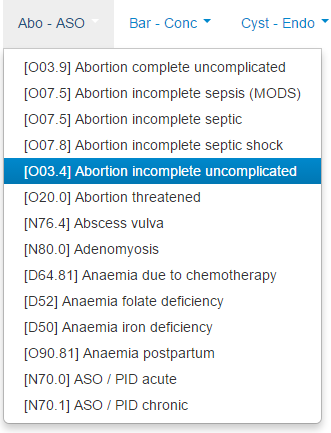
\includegraphics[width=0.3\textwidth]{Graphics/Screenshots/formsHelperDropdown}}}
				\caption{ICD 10 Codes Dropdown.}
		  		\label{fig:forms3}
			\end{figure}
			\item Fill in relevant ICD code into the input box
			\item Add extra field if more codes are needed.
			\item Repeat 1 and 2 as much as needed.
		\end{enumerate}
\subsection{Statistics Queries}
	\begin{figure}[H]
		\centerline{\fbox{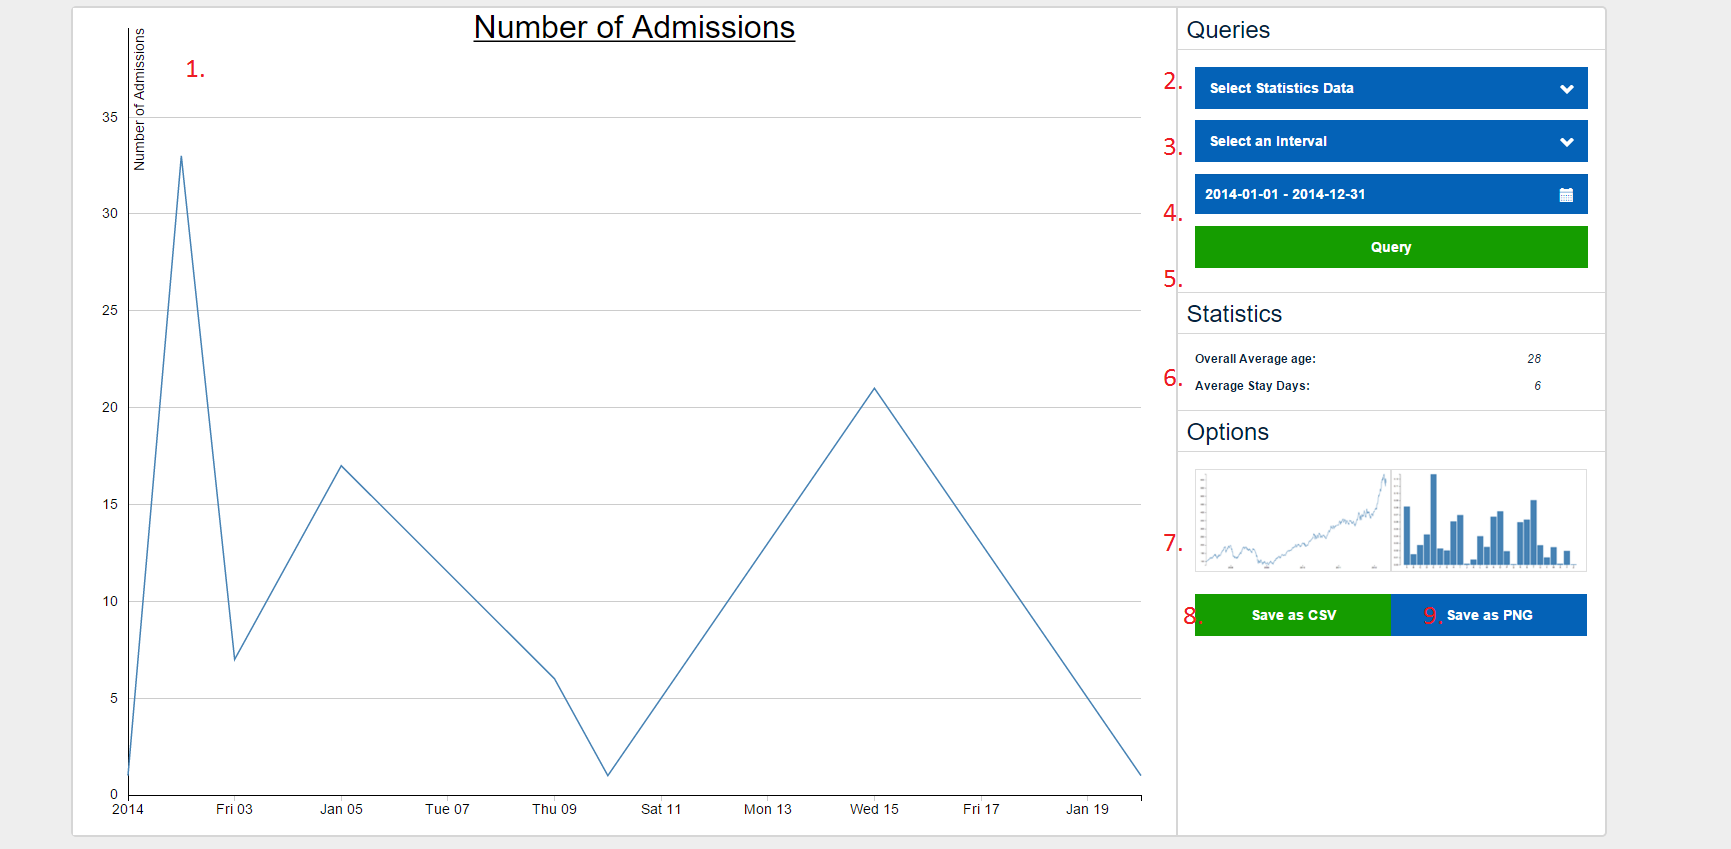
\includegraphics[width=1.0\textwidth]{Graphics/Screenshots/statsQuery}}}
		\caption{Statisical Queries Page.}
  		\label{fig:statsQ1}
	\end{figure}
	\subsubsection{Description} This page allows the administrative user to query statistics to obtain information for research purposes.
	\subsubsection{Detailed Component Description}
		\begin{enumerate}
			\item \textbf{Statistics Graph:} This is the graph that represents the statistics data queried. The default graph show upon page load is always the number of admissions over a daily interval. 
			\item \textbf{Statistics Data Dropdown List:} This is a dropdown list that allows the user to select the data they would like to query.
			\item \textbf{Interval Dropdown List:} This is a dropdown list that allows the user to select the interval they would like the data to be grouped by.
			\item \textbf{Date Selector:} This is a selection input box that allows the user to choose the period in which they want the data from. Eg. They would choose a start date of 01/01/2014 up until an end date of 31/10/2014.
			\item \textbf{Query Button:} This button can be clicked to create a new statistics graph with options selected by user.
			\item \textbf{Statistics Average Section:} This section contains averages for certain statistics collected.
			\item \textbf{Graph Type Selector: } This is two selectors that allow the user to choose whether the information is showed as a bar graph or a line graph.
			\item \textbf{Save as CSV:} This allows the user to save the data represented into a CSV file.
			\item \textbf{Save as PNG:} This allows the user to save the data represented as a PNG image file.
		\end{enumerate}
	\subsubsection{How to query statistics:}
		\begin{enumerate}
			\item Select the statistics data from the statistics data dropdown list. An example of the dropdown list in use is shown in figure \ref{fig:statsQ2}.
			\begin{figure}[H]
				\centerline{\fbox{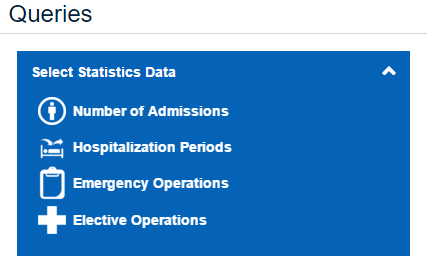
\includegraphics[width=0.4\textwidth]{Graphics/Screenshots/statisticsData}}}
				\caption{Statistics Data Dropdown List in use.}
  				\label{fig:statsQ2}
			\end{figure}
			\item Select the interval period from the interval dropdown list. An example of the dropdown list in use is show in figure \ref{fig:statsQ3}.
			\begin{figure}[H]
				\centerline{\fbox{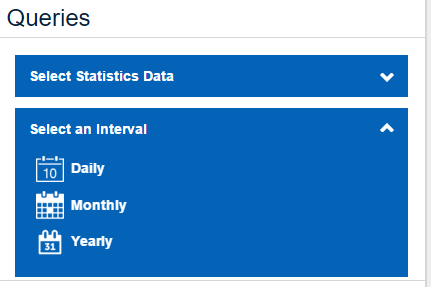
\includegraphics[width=0.4\textwidth]{Graphics/Screenshots/intervalData}}}
				\caption{Interval Dropdown List in use.}
  				\label{fig:statsQ3}
			\end{figure}
			\item Select the start and end dates from the Date Selector(Always start with the start date). An example of start and end dates selected is shown in figure \ref{fig:statsQ4}
			\begin{figure}[H]
				\centerline{\fbox{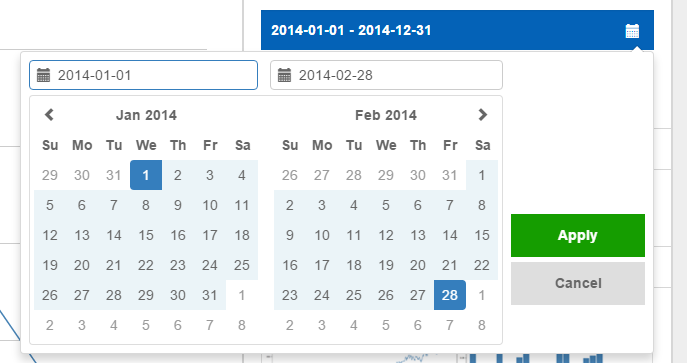
\includegraphics[width=0.4\textwidth]{Graphics/Screenshots/dateSelection}}}
				\caption{Statistics Data Dropdown List in use.}
  				\label{fig:statsQ4}
			\end{figure}
			\item Click on the query button and the new graph with the options selected will be shown.
		\end{enumerate}
	\subsubsection{How to select the graph type}
		\begin{enumerate}
			\item Choose either the bar or line graph from the Graph type selector
		\end{enumerate}
	\subsubsection{How to save graph as CSV}
		\begin{enumerate}
			\item Click on the save as CSV button.
		\end{enumerate}
	\subsubsection{How to save graph as PNG}
		\begin{enumerate}
			\item Click on the save as PNG button.
		\end{enumerate}
	\subsubsection{How to select the graph type}
		\begin{enumerate}
			\item Choose either the bar or line graph from the Graph type selector
		\end{enumerate}
\subsection{Statistics Dashboard}
	\begin{figure}[H]
		\centerline{\fbox{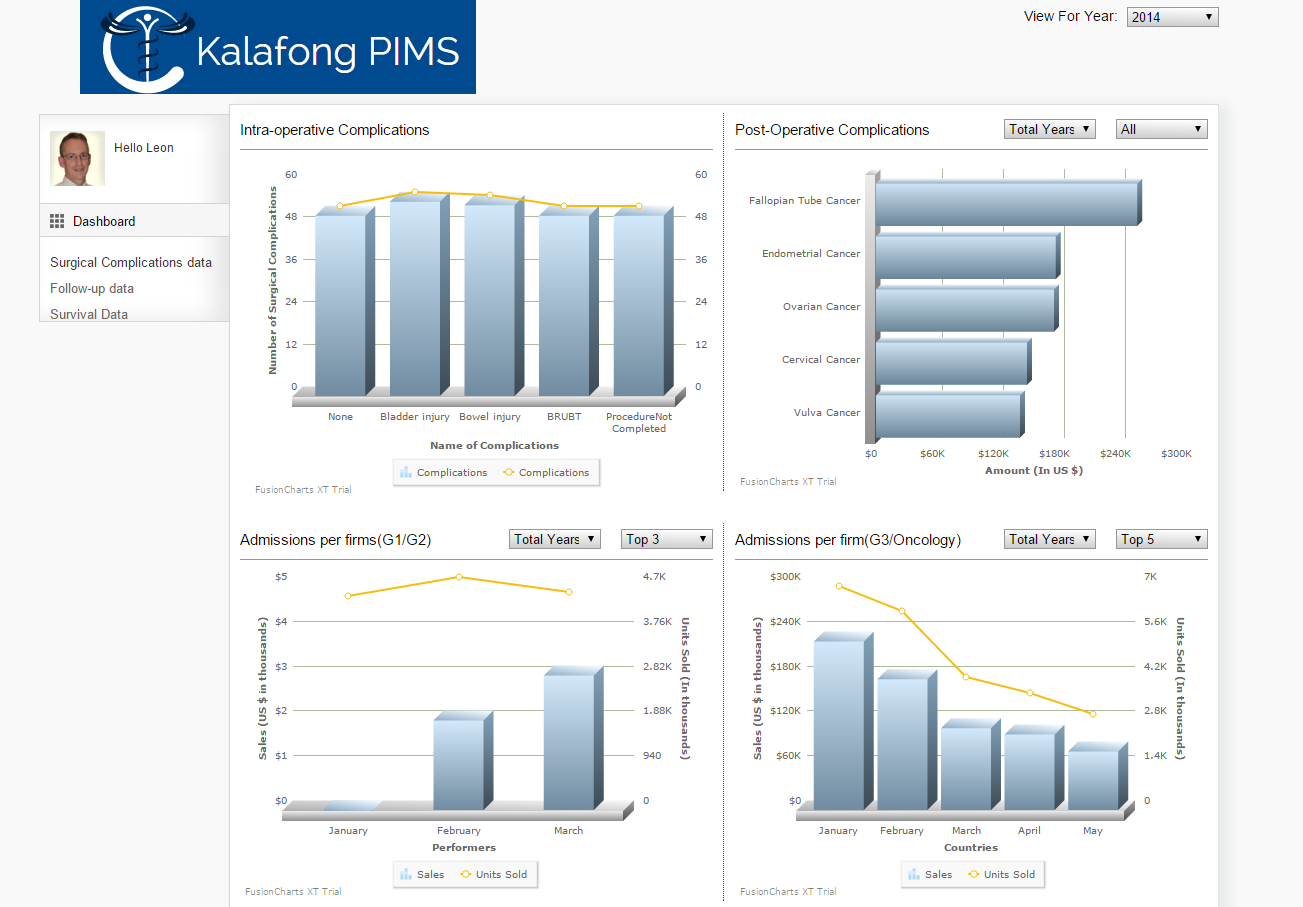
\includegraphics[width=1.0\textwidth]{Graphics/Screenshots/dashboard}}}
		\caption{The Statistics Dashboard.}
  		\label{fig:dash1}
	\end{figure}
	\subsubsection{Description} This dashboard is available to the admin user and allows them to an overall summary of multiple graphs.
	\subsubsection{Detailed Component Description}
		\begin{enumerate}
			\item \textbf{Dashboard Sections:} This section of the dashboard allows the user to view graphs grouped into their respective sections. 
			\item \textbf{Graph:} This is a graph that represents certain data.
			\item \textbf{Year selector: } This allows the user to select what year the graphs data represents.
			\item \textbf{Total Years Selector: }  This allows the user to select the years for that specific graph.
			\item \textbf{Top Selector:} This allows the user to choose whether the graph shows the Top 5 statistics or all of them.
		\end{enumerate}
	\subsubsection{How to select the top 5 of a specific graph.}
		\begin{enumerate}
			\item Click on the top selector and choose the top 5 from the dropdown list.
		\end{enumerate}
\subsection{Add User}
	\begin{figure}[H]
		\centerline{\fbox{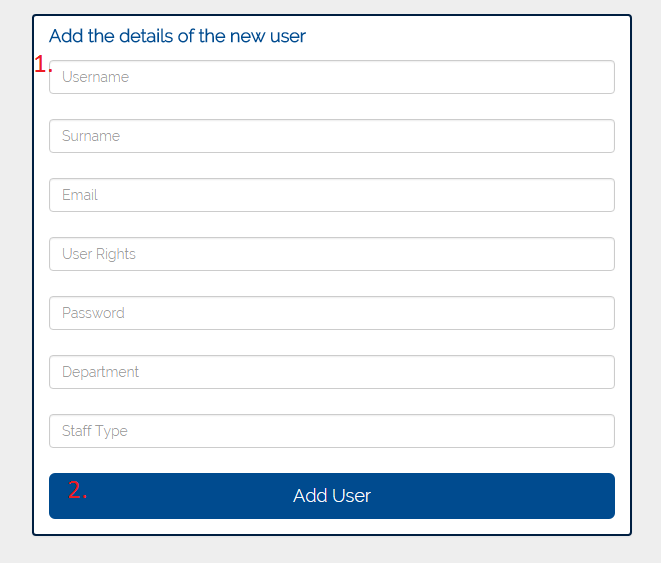
\includegraphics[width=0.8\textwidth]{Graphics/Screenshots/addUser}}}
		\caption{The Add User Box}
  		\label{fig:addUser}
	\end{figure}
	\subsubsection{Description} This is the add user input box which allows the admin user to add users that can log into the system and perform certain responsibilities.
	\subsubsection{Detailed Component Description}
		\begin{enumerate}
			\item \textbf{Input box:} This is an input box in which the user can fill the neccessary information in the box.
			\item \textbf{Add User Button:} This button when clicked will take all the information from the form and use it to add a user to the system.
		\end{enumerate}
	\subsubsection{How to add a user}
		\begin{enumerate}
			\item Fill in the user's name
			\item Fill in the user's surname
			\item Fill in the user's email(must be valid)
			\item Fill in the user's rights (1 for admin, 0 for regular user)
			\item Fill in the user's password
			\item Fill in the user's department (Must be a valid department)
			\item Fill in the user's staff type (Must be a valid staff type)
		\end{enumerate}
\subsection{Remove User}
	\begin{figure}[H]
		\centerline{\fbox{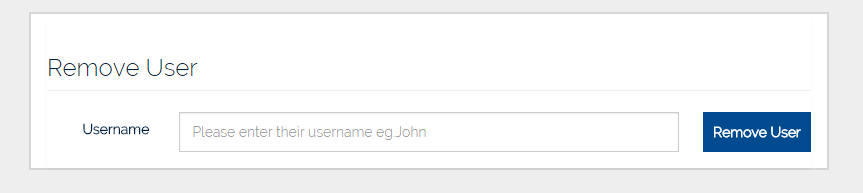
\includegraphics[width=0.8\textwidth]{Graphics/Screenshots/removeUser}}}
		\caption{The Remover User Form.}
  		\label{fig:removeUser1}
	\end{figure}
	\subsubsection{Description} This section allows an admin user to remove a user from the system.
	\subsubsection{Detailed Component Description}
		\begin{enumerate}
			\item \textbf{Username input box:} This input box is where the admin user specifies the username of the user to be removed from the system.
			\item \textbf{Remove user button:} This button when clicked the username specified is valid will remove the user from the database.
		\end{enumerate}
	\subsubsection{How to remove a user}
		\begin{enumerate}
			\item Fill in a valid user name in the username input box.
			\item Click on the remove user button.
		\end{enumerate}
\subsection{Update Profile}
	\begin{figure}[H]
		\centerline{\fbox{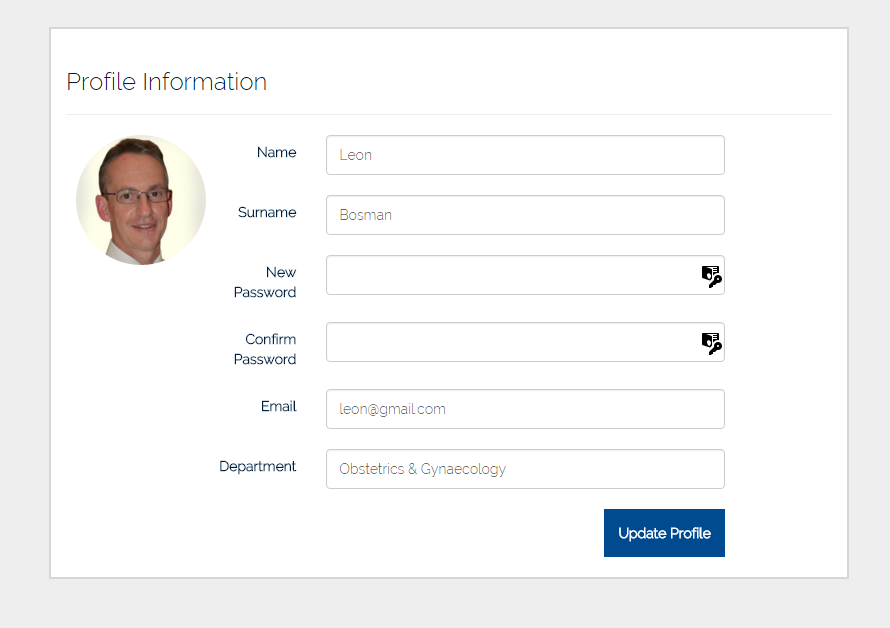
\includegraphics[width=0.8\textwidth]{Graphics/Screenshots/profileInformation}}}
		\caption{The Update Profile Page}
  		\label{fig:navbar4}
	\end{figure}
	\subsubsection{Description} 
	\subsubsection{Detailed Component Description}
		\begin{enumerate}
			\item \textbf{Username input box:} This input box is where the admin user specifies the username of the user to be removed from the system.
			\item \textbf{Remove user button:}
		\end{enumerate}
	\subsubsection{How to\ldots}
		\begin{enumerate}
			\item Some stuff \ldots
		\end{enumerate}
\subsection{Predict}
	\begin{figure}[H]
		\centerline{\fbox{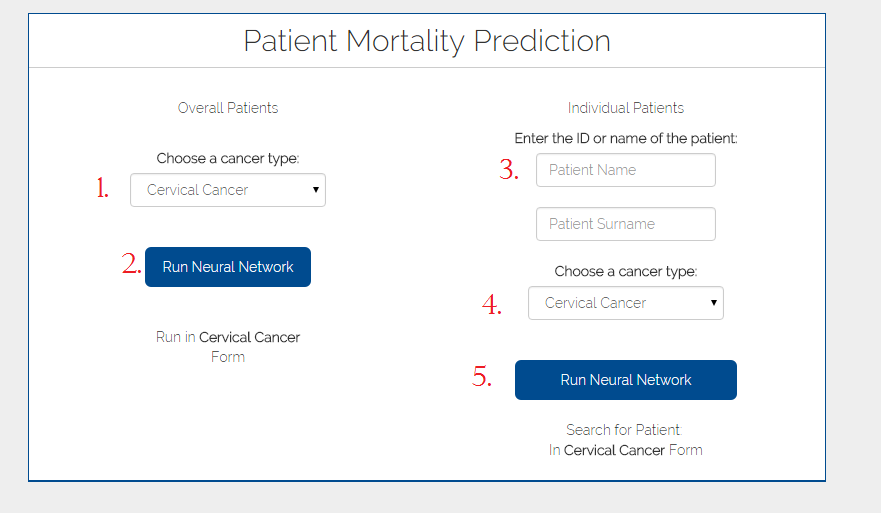
\includegraphics[width=0.8\textwidth]{Graphics/Screenshots/predict}}}
		\caption{The User Navbar.}
  		\label{fig:navbar4}
	\end{figure}
	\subsubsection{Description}
	\subsubsection{Detailed Component Description}
		\begin{enumerate}
			\item \textbf{Some stuff:} 
		\end{enumerate}
	\subsubsection{How to\ldots}
		\begin{enumerate}
			\item Some stuff \ldots
		\end{enumerate}
\subsection{Tutorial}
	\begin{figure}[H]
		\centerline{\fbox{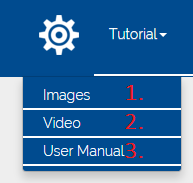
\includegraphics[width=0.3\textwidth]{Graphics/Screenshots/tutorialDropdown}}}
		\caption{The User Navbar.}
  		\label{fig:navbar4}
	\end{figure}
	\subsubsection{Description}
	\subsubsection{Detailed Component Description}
		\begin{enumerate}
			\item \textbf{Some stuff:} 
		\end{enumerate}
	\subsubsection{How to\ldots}
		\begin{enumerate}
			\item Some stuff \ldots
		\end{enumerate}
\newpage


\section{Using the System}
\begin{description}
\item The login, forms, user and statistics operations are described in this chapter.
\end{description}


\subsection{User}
	  
\subsubsection{add user}
\begin{description}
\item [Functional Description] This operation adds a user to the PENTEC-PIMS database.
\item [Formal Description] \hfill
\begin{itemize}
	\item Syntax: add user (username,surname,password,staff type,department,email address,user right) as [Users] [A schema to save the details of all medical staff that can access the system]\\
	\item Parameters:
		\begin{itemize}
			\item [schema] (Required when chosen) : Users Schema\\
			\item [pentec\_pims] (Required) : This is the name of the database in mongoose that we are using\\
			\item [details](Required):All the above mentioned details in syntax are important to add a user\\
		 \end{itemize}
\end{itemize}
\item[Examples]\hfill
\begin{itemize}
	\item add user John Doe, Medical Intern, User right 2, Gynaecologist
	\item add user url:http://kalafongpims.herokuapp.com/addUser
	\item URL : :http://kalafongpims.herokuapp.com as Medical Staff This is a medical research dataset PENTEC Software User Manual 0.1.0 14
\end{itemize}
\item[Possible errors]\hfill
	\begin{itemize}
	\item You do not have the login creditials
	\item A user with name [username]already exists
	\item You don't have the role of admin
	\end{itemize}
\item[Solutions]\hfill
	\begin{itemize}
	\item Go to admin(Dr Snyman) and request he add you to the database of users.
	\item Register with your already given details. No duplicates allowed.
	\item  Go to admin(Dr Snyman) and request he make you admin.
	\end{itemize}
\item[Related operations] remove user
\end{description}
	  
\subsubsection{edit profile}
\begin{description}
\item[Functional Description] This operation edits a users profile and saves it to the PENTEC-PIMS database.
\item[Formal description]\hfill
\begin{itemize}
	\item Syntax: edit user (username,surname,password,confirm password,staff type,department,email address,user right) as [Users] [A schema to save the details of all medical staff that can access the system]\\
	\item Parameters:
		\begin{itemize}
			\item [schema] (Required when chosen) : Users Schema
			\item [pentec\_pims] (Required) : This is the name of the database in mongoose that we are using.
			\item [details] (Required) :All the above mentioned details in syntax are important to complete edit profile.
		\end{itemize}
\end{itemize}

\item[Examples]\hfill
\begin{itemize}
	\item edit user John Doe, Medical Intern, User right 2, Gynaecologist
	\item edit user url:http://kalafongpims.herokuapp.com/editProfile
	\item URL : :http://kalafongpims.herokuapp.com as Medical Staff This is a medical research dataset PENTEC Software User Manual 0.1.0 14
\end{itemize}

\item[Possible errors]\hfill
\begin{itemize}
	\item You do not have the login creditials to log into the system
	\item Passwords don't match
	\item You don't have the role of admin
	\item You do not appear on the system
\end{itemize}

\item[Solutions]\hfill
\begin{itemize}
	\item Go to admin(Dr Snyman) and request he add you to the database of users.
	\item Register with your already given details sent to your email. No duplicates allowed.
	\item Re-enter your password
	\item  Go to admin(Dr Snyman) and request he make you admin.
\end{itemize}
\item[Related operations] add user
\end{description}
		   
\subsubsection{password}
\begin{description}
\item[Functional description] This operation changes your password on the PENTEC-PIMS database.
\item[Formal description]\hfill
\begin{itemize}
	\item Syntax:password (confirm password, password) as [Users] [A schema to save the details of all medical staff that can access the system]\\
	\item Parameters:
	\begin{itemize}
		\item [schema] (Required when chosen) : Users Schema
		\item [pentec\_pims] (Required) : This is the name of the database in mongoose that we are using.
		\item [details] (Required) :All the above mentioned details in syntax are important to complete password.
	\end{itemize}
\end{itemize}

\item[Examples]\hfill
\begin{itemize}
	\item password mysecretpassword, mysecretpassword
	\item add user url:http://kalafongpims.herokuapp.com/editProfile
	\item URL : :http://kalafongpims.herokuapp.com as Medical Staff This is a medical research dataset
	PENTEC Software User Manual 0.1.0 14
\end{itemize}
\item[Possible errors]\hfill
\begin{itemize}
	\item You do not have the login creditials
	\item You don't have the role of admin
	\item Passwords dont match
\end{itemize}
\item[Solutions]\hfill
\begin{itemize}
	\item Go to admin(Dr Snyman) and request he add you to the database of users.
	\item  Go to admin(Dr Snyman) and request he make you admin.
	\item Re-enter your password carefully.
\end{itemize}
\item[Related operations] none
\end{description}

\subsubsection{list for}
\begin{description}
\item[Functional description] This operation list all the available forms in the PENTEC-PIMS database.
\item[Formal description]\hfill
\begin{itemize}
	\item Syntax: list form (form name) as [Forms] [A schema to save the details of all medical forms in the system]\\
	\item Parameters:
	\begin{itemize}
		\item [schema] (Required when chosen) : Forms Schema
		\item [pentec\_pims] (Required) : This is the name of the database in mongoose that we are using.
		\item [details] (Required) :All the above mentioned details in syntax are important to complete list form.
	\end{itemize}
\end{itemize}

\item[Examples]\hfill
\begin{itemize}
	\item list form Gynaecology Form
	\item list form url:http://kalafongpims.herokuapp.com/forms
	\item URL : :http://kalafongpims.herokuapp.com as Medical Staff This is a medical research dataset
	PENTEC Software User Manual 0.1.0 14
\end{itemize}

\item[Possible errors]\hfill
\begin{itemize}
	\item You do not have the login creditials
	\item The form you are looking for does not exist
\end{itemize}

\item[Solutions]\hfill
\begin{itemize}
	\item Go to admin(Dr Snyman) and request he add you to the database of users.
	\item Go to admin(Dr Snyman) and request he create the form.
\end{itemize}
\item[Related operations] none

\end{description}
	      	      
	      
\subsubsection{save form}
\begin{description}
\item[Functional description] This operation allows you to save a form to the PENTEC-PIMS database.
\item [Formal description]\hfill
\begin{itemize}
	\item Syntax: save form (data, form name) as [Forms] [A schema to save the details of all forms created in the system]\\
	\item Parameters:
	\begin{itemize}
		\item [schema] (Required when chosen) : Forms Schema
		\item [pentec\_pims] (Required) : This is the name of the database in mongoose that we are using.
		\item [details] (Required) :All the above mentioned details in syntax are important to complete save form.
	\end{itemize}
\end{itemize}

\item[Examples]\hfill
\begin{itemize}
	\item save form discharge form, JSON Object
	\item save form url:http://kalafongpims.herokuapp.com/formbuilder
	\item URL : :http://kalafongpims.herokuapp.com as Medical Staff This is a medical research dataset
	PENTEC Software User Manual 0.1.0 14
\end{itemize}

\item[Possible errors]none
\item[Solutions] none
\item [Related operations] list form, add form
\end{description}

\subsubsection{send notification}
\begin{description}
\item[Functional description] This operation allows you to notify a patient of their follow up via email.
\item[Formal description]\hfill
\begin{itemize}
	\item Syntax: add notification (username, email, message, date) as [Users] [A schema to save the details of all medical staff that can access the system]\\
	\item Parameters:
	\begin{itemize}
		\item [schema] (Required when chosen) : Users Schema
		\item [pentec\_pims] (Required) : This is the name of the database in mongoose that we are using.
		\item [details] (Required) :All the above mentioned details in syntax are important to complete send notification.
	\end{itemize}
\end{itemize}
\item[Examples]\hfill
\begin{itemize}
	\item add notification John Doe,john@gmail.com, "John Please come for your checkup",2015
	\item add notification url:http://kalafongpims.herokuapp.com/sendNotification
	\item URL : :http://kalafongpims.herokuapp.com as Medical Staff This is a medical research dataset
	PENTEC Software User Manual 0.1.0 14
\end{itemize}

\item[Possible errors]\hfill
\begin{itemize}
	\item You cant find the users name
	\item User does not have an email address
\end{itemize}


\item[Solutions]\hfill
\begin{itemize}
	\item Patient does not exist in the system
	\item Notification cannot be sent to user
\end{itemize}


\item[Related operations] remove user
\end{description}
	   
\subsubsection{list department}
\begin{description}
\item[Functional description] This operation lists all the departments on the splash screen from the PENTEC-PIMS database.
\item[Formal description]\hfill
\begin{itemize}
	\item Syntax: list department (name of department, link) as [Departments] [A schema to save the details of all departments in the system and display them on the splash screen]\\
	\item Parameters:
	\begin{itemize}
		\item [schema] (Required when chosen) : Departments Schema
		\item [pentec\_pims] (Required) : This is the name of the database in mongoose that we are using.
		\item [details] (Required) :All the above mentioned details in syntax are important to complete list user.
	\end{itemize}
\end{itemize}

\item[Examples]\hfill
\begin{itemize}
	\item list department Gynaecology, www/d/
	\item list department url:http://kalafongpims.herokuapp.com/splash
	\item URL : :http://kalafongpims.herokuapp.com as Medical Staff This is a medical research dataset
	PENTEC Software User Manual 0.1.0 14
\end{itemize}
\item[Possible errors] None
\item[Solutions] None
\item[Related operations] none
\end{description}
	      
\subsubsection{exit}
\begin{description}
\item[Functional description] This operation adds a user to the PENTEC-PIMS database.
\item[Formal description]\hfill
\begin{itemize}
	\item Syntax: add user (none) as [none] [none]\\
	\item Parameters:
	\begin{itemize}
		\item [schema] (Required when chosen) : Users Schema
		\item [pentec\_pims] (Required) : This is the name of the database in mongoose that we are using.
		\item [details] (Required) :All the above mentioned details in syntax are important to complete exit.
	\end{itemize}
\end{itemize}

\item[Examples]\hfill
\begin{itemize}
	\item exit [press logout button]
	\item exit url:http://kalafongpims.herokuapp.com/home
	\item URL : :http://kalafongpims.herokuapp.com as Medical Staff This is a medical research dataset
	PENTEC Software User Manual 0.1.0 14
\end{itemize}

\item[Possible errors] none
\item[Solutions] none
\item [Related operations] login
\end{description}

\subsection{Login}
\subsubsection{authenticate} 
\begin{description}
\item[Functional Description] This function authenticates a user and logs them into the system.
\item[Formal Description]\hfill
\begin{itemize}
	\item Syntax: authenticate([username], [password], [callback])\\
	\item Parameters:
		\begin{itemize}
			\item [username] (Required): This is the username of the user, it will usually be the user's name or a unique number assigned to them.
			\item [password] (Required): This is the password of the user and is used to authenticate the user.
			\item [callback](Opitional): This is the callback function and is used to keep the processes synchronous.
		\end{itemize}
\end{itemize}
\item[Examples]\hfill
\begin{itemize}
	\item authenticate("John", 1234)
	\item authenticate("john", 1234, thisIsAFunction(){})
\end{itemize}
\item[Possible Errors \&  Solutions]\hfill
	\begin{itemize}
		\item Problem: Your login does not exist.
		\item Solution: Contact supervisor.
		\item Problem: Your password is incorrect.
		\item Solution: Contact supervisor.
		\item Problem: You are trying to access an admin page but it takes you to a regular user page.
		\item Solution: Request supervisor to change your rank.
	\end{itemize}
\item [Related operations]	checkAdmin
\end{description}

\subsubsection{check admin}
\begin{description}
\item[Functional Description] Determines if the user is an administrator.
\item[Formal Description]\hfill
\begin{itemize}
	\item Syntax: checkAdmin([username], [password], [callback])\\
	\item Parameters:
		\begin{itemize}
			\item [username] (Required): This is the username of the user, it will usually be the user's name or a unique number assigned to them.
			\item [password] (Required): This is the password of the user and is used to authenticate the user.
			\item [callback](Opitional): This is the callback function and is used to keep the processes synchronous.
		\end{itemize}
\end{itemize}
\item[Examples]\hfill
\begin{itemize}
	\item checkAdmin("John", 1234)
	\item checkAdmin("john", 1234, thisIsAFunction(){})
\end{itemize}
\item[Possible Errors \& Solutions]
\begin{itemize}
	\item Problem: You are trying to access an admin page but takes you to a regular user page.
	\item Solution: Request supervisor to change your rank.
\end{itemize}
\item[Related operations] authenticate
\end{description}

\subsubsection{recaptcha}
\begin{description}
\item[Functional Description] This function is a security feature to ensure the user is not an automated bot or machine.
\item[Formal Description]\hfill
\begin{itemize}
	\item Syntax: recapture([action], [callback])\\
	\item Parameters:
		\begin{itemize}
			\item [action] (Required): This is the action taken by the user in the form of a check on the checkbox.
			\item [callback](Opitional): This is the callback function and invoked by the click event and allows the user to log into the system.
		\end{itemize}
\end{itemize}
\item[Examples]\hfill
\begin{itemize}
	\item recaptcha(event(Click), thisIsACallbackFunction(){//allow user to log in})
\end{itemize}
\item[Possible Errors \& Solutions]
\begin{itemize}
	\item Problem: Error message "Please check the recaptcha box before logging in"
	\item Solution: Locate the recaptcha box at the bottom of the log in box and click it.
\end{itemize}
\item[Related operations] authenticate
\end{description}


\subsection{Statistics}

\subsubsection{get daterange}
\begin{description}
\item[Functional Description] This function allows the user to select a time period that he would like his data to reflect.
\item[Formal Description]/hfill
\begin{itemize}
	\item Syntax: getDatarange([startDate], [endDate], [callback])\\
	\item Parameters:
		\begin{itemize}
			\item [startDate](Required) This is the start date that has been selected.
			\item [endDate](Required) This is the end date that has been selected.
			\item [callback](Optional) This is the callback function and is used to keep the processes synchronous.
		\end{itemize}
\end{itemize}
\item[Examples]\hfill
\begin{itemize}
	\item getDatarange({startDate : "10/10/2014", endDate: "10/10/2015"})
	\item getDatarange({startDate : "10/10/2014", endDate: "10/10/2015"}, callback)
\end{itemize}
\item[Possible Errors \& Solutions]
\begin{itemize}
	\item Problem: No date selected
	\item Solution: Reselect the date on the date time picker and click apply then select other procedures and click query.
	\item Problem: No procedures in the dates selected
	\item Solution: Graph will show user there are no procedures in that period.
\end{itemize}
\item[Related operations] \hfill
\begin{itemize}
	\item get interval
	\item get graph
\end{itemize}
\end{description}

\subsubsection{get interval}
\begin{description}
\item[Functional Description] This function gets the interval based data in the dropdownlist and certain selectors and uses it to query the database.
\item[Formal Description]/hfill
\begin{itemize}
	\item Syntax: getInterval([selectors], [callback])\\
	\item Parameters:
		\begin{itemize}
			\item [interval][statistics],[selectors](Required) These are the selectors put in place to customize the procedures that are selected.
			\item [callback](Required) This is the callback function and is used to keep the processes synchronous.
		\end{itemize}
\end{itemize}
\item[Examples]\hfill
\begin{itemize}
	\item getInterval(Weekly,Average Age,{startDate : "10/10/2014", age: 25, endDate: "10/10/2015"})
	\item getInterval(Yearly, Average Age,{startDate : "10/10/2014", age: 25, endDate: "10/10/2015"}, callback)
\end{itemize}
\item[Possible Errors \& Solutions]
\begin{itemize}
	\item Problem: Invalid selectors
	\item Solution: Choose a valid selector.
	\item Problem: No operations during that selector
	\item Solution: Graph will correctly depict the scenario.
\end{itemize}
\item[Related operations] \hfill
\begin{itemize}
	\item get daterange
	\item get graph
\end{itemize}
\end{description}

\subsubsection{get graph}

\begin{description}
\item[Functional Description] This function gets data selected from the input boxes and after querying the database returns them in a format which can be converted into a graph.
\item[Formal Description]/hfill
\begin{itemize}
	\item Syntax: getGraph([startDate],[endDate],[interval],[statistic], [callback])\\
	\item Parameters:
		\begin{itemize}
			\item [startDate](Required) This is the start date that has been selected.
			\item [endDate](Required) This is the end date that has been selected.
			\item [interval](Required) This is the interval that has been selected.
			\item [statistic](Required) This is the statistic that has been selected.
			\item [callback](Optional) This is the callback function and is used to keep the processes synchronous.
		\end{itemize}
\end{itemize}
\item[Examples]\hfill
\begin{itemize}
	\item getGraph({startDate : "10/10/2014", procedure: "all", endDate: "10/10/2015"},"Weekly", "Average Age", )
	\item getGraph({startDate : "10/10/2014", procedure: "all" ,endDate: "10/10/2015"}, callback)
\end{itemize}
\item[Possible Errors \& Solutions]
\begin{itemize}
	\item Problem: Data does not exist
	\item Solution: Graph shows the appropriate message.
	\item Problem: Invalid selectors
	\item Solution: Choose a valid selector.
\end{itemize}
\item[Related operations] \hfill
\begin{itemize}
	\item get interval
	\item get datarange
\end{itemize}
\end{description}

\subsubsection{get statistics}
\begin{description}
\item[Functional Description] This function allows the user to select a specific statistic he would like his data to reflect.
\item[Formal Description]/hfill
\begin{itemize}
	\item Syntax: getStatistics([stats], [callback])\\
	\item Parameters:
		\begin{itemize}
			\item [stats](Required) This is the statistics that has been selected.
			\item [callback](Optional) This is the callback function and is used to keep the processes synchronous.
		\end{itemize}
\end{itemize}
\item[Examples]\hfill
\begin{itemize}
	\item getStatistics({stats:"Elective Procedures"})
\end{itemize}
\item[Possible Errors \& Solutions]
\begin{itemize}
	\item Problem: No statistic value selected
	\item Solution: Error message asking you to select a statistic value will show.
	\item Problem: No procedures in the dates selected
	\item Solution: Graph will show user there are no procedures in that period and ask you to select dates.
\end{itemize}
\item[Related operations] \hfill
\begin{itemize}
	\item get interval
	\item get graph
	\item get daterange
\end{itemize}
\end{description}
\newpage

\section{Troubleshooting}
\subsection{Introduction}
This section contains a series of tables that describe
possible solutions to problems that may occur when
using your PC. Each table contains: \\
\begin{itemize}
	\item Symptoms that describe the sign or warning message for the type of problem.
	\item Possible solutions that describe what you should
do to try to solve the problem. 
\end{itemize}

\setlength{\arrayrulewidth}{1mm}
\setlength{\tabcolsep}{18pt}
\renewcommand{\arraystretch}{1.5}
 

\begin{tabular}{ |p{3cm}|p{3cm}|  }
\hline
\multicolumn{2}{|c|}{Troubleshooting} \\
\hline
Symptoms & Possible solution \\
\hline
You press the login button and nothing happens & 1. You entered the wrong username/password combination. 1.1 Click show password to see what you have typed. 1.2 Recheck your email from admin to ensure you are using the correct username/password combination. 1.3 You have not clicked the recaptcha box. \\
Aland Islands & AX. 1.4 You have not entered a username or password. \\
Cannot add new user & 2. You have to fill all the textboxes\\
Cannot edit profile    &Make sure you have internet connection  \\
Cannot query statistics & Make sure you have selected an option for each dropdownlist. Ensure you have clicked the query button.  \\
\hline
\end{tabular}


\end{document}